\documentclass[10pt,a4paper,twocolumn,twoside]{article}
\usepackage[utf8]{inputenc}
\usepackage[catalan]{babel}
\usepackage{multicol}
\usepackage{graphicx}
\usepackage{fancyhdr}
\usepackage{times}
\usepackage{titlesec}
\usepackage{multirow}
\usepackage{lettrine}
\usepackage{hyperref}
\usepackage{enumitem}
\usepackage{pgfgantt}
\usepackage{needspace}
\usepackage[top=2cm, bottom=1.5cm, left=2cm, right=2cm]{geometry}
\usepackage[figurename=Fig.,tablename=TAULA]{caption}
\captionsetup[table]{textfont=sc}

\hypersetup{
    colorlinks=true,
    linkcolor=black,
    filecolor=black,      
    urlcolor=blue,
    citecolor=black
}

\author{\LARGE\sffamily Narcís Nogué Bonet}
\title{\Huge{\sffamily Aterratge autònom d'avions model basat en visió}}
\date{}

\newcommand\blfootnote[1]{%
  \begingroup
  \renewcommand\thefootnote{}\footnote{#1}%
  \addtocounter{footnote}{-1}%
  \endgroup
}

%
%\large\bfseries\sffamily
\titleformat{\section}
{\large\sffamily\scshape\bfseries}
{\textbf{\thesection}}{1em}{}

\begin{document}

\fancyhead[LO]{\scriptsize NARCÍS NOGUÉ BONET}
\fancyhead[RO]{\thepage}
\fancyhead[LE]{\thepage}
\fancyhead[RE]{\scriptsize ATERRATGE AUTÒNOM D'AVIONS MODEL BASAT EN VISIÓ}

\fancyfoot[CO,CE]{}

\fancypagestyle{primerapagina}
{
   \fancyhf{}
   \fancyhead[L]{\scriptsize TFG EN ENGINYERIA INFORMÀTICA, ESCOLA D'ENGINYERIA (EE), UNIVERSITAT AUTÒNOMA DE BARCELONA (UAB)}
   \fancyfoot[C]{\scriptsize Març de 2021, Escola d'Enginyeria (UAB)}
}

%\lhead{\thepage}
%\chead{}
%\rhead{\tiny EE/UAB TFG INFORMÀTICA: TÍTOL (ABREUJAT SI ÉS MOLT LLARG)}
%\lhead{ EE/UAB \thepage}
%\lfoot{}
%\cfoot{\tiny{February 2015, Escola d'Enginyeria (UAB)}}
%\rfoot{}
\renewcommand{\headrulewidth}{0pt}
\renewcommand{\footrulewidth}{0pt}
\pagestyle{fancy}

%\thispagestyle{myheadings}
\twocolumn[\begin{@twocolumnfalse}

%\vspace*{-1cm}{\scriptsize TFG EN ENGINYERIA INFORMÀTICA, ESCOLA D'ENGINYERIA (EE), UNIVERSITAT AUTÒNOMA DE BARCELONA (UAB)}

\maketitle

\thispagestyle{primerapagina}
%\twocolumn[\begin{@twocolumnfalse}
%\maketitle
%\begin{abstract}
\begin{center}
\parbox{0.915\textwidth}
{\sffamily
\textbf{Introducció--}
Com indica el títol, el meu Treball de Final de Grau consisteix a crear un
sistema de control autònom que sigui capaç d'aterrar un avió en una pista
d'aterratge utilitzant únicament una càmera i altres sensors bàsics com
acceleròmetres i giroscopis. Actualment la majoria de sistemes d'aterratge
autònom necessiten modificacions substancials de la pista d'aterratge per instal·lar
un sistema ILS (Instrument Landing System), dissenyat per permetre a una aeronau
aterrar de nit o en baixa visibilitat. Tot i això, hi ha un subgrup important dels
aeroports que segueixen les normes VFR (Visual Flight Rules), on només es pot
aterrar de dia i quan la visibilitat sigui suficient, ja que l'única informació
que té el pilot és el contacte visual directe de la pista d'aterratge. La
majoria d'aeroports petits, aeròdroms i pistes de muntanya cauen en aquesta categoria,
i per tant l'aterratge autònom per mètodes convencionals hi és de moment impossible.
La solució que proposo deriva directament d'aquesta restricció: si la majoria
de pistes d'aterratge estan pensades i dissenyades per a vol visual, un sistema
d'aterratge autònom ha de ser capaç d'aterrar de forma purament visual, i sense
confiar en cap input des de la pista d'aterratge, per a poder-se considerar plenament
autònom i genèric.
\\
%\end{abstract}
\\
}

{\vrule depth 0pt height 0.5pt width 4cm\hspace{7.5pt}%
\raisebox{-3.5pt}{\fontfamily{pzd}\fontencoding{U}\fontseries{m}\fontshape{n}\fontsize{11}{12}\selectfont\char70}%
\hspace{7.5pt}\vrule depth 0pt height 0.5pt width 4cm\relax}

\end{center}

\bigskip
\end{@twocolumnfalse}]

\blfootnote{$\bullet$ E-mail de contacte: nnogue4@gmail.com}
\blfootnote{$\bullet$ Menció realitzada: Computació}
\blfootnote{$\bullet$ Treball tutoritzat per: Felipe Lumbreras Ruiz (Department of Computer Science)}
\blfootnote{$\bullet$ Curs 2020/21}

\section{Objectius}

\lettrine[lines=3]{P}{er} la naturalesa del projecte, els objectius del meu Treball de Final de Grau poden
augmentar en complexitat molt ràpidament, i per tant els dividiré en dues seccions: els objectius necessaris per tenir un
MVP (Minimum Viable Product), i la resta d'objectius opcionals per seguir expandint el projecte més enllà.

Objectius per a un MVP:
\begin{itemize}
  \item Dissenyar i implementar un algoritme de control capaç d'aterrar un avió model si sap on és la pista d'aterratge.
  \item Dissenyar una simulació prou acurada d'un cas genèric d'aterratge, sobre la qual poder provar els algoritmes de control i de detecció de la pista.
  \item Dissenyar i implementar una xarxa neuronal capaç de reconèixer qualsevol pista d'aterratge sobre la qual hagi estat entrenada directament.
\end{itemize}
Objectius addicionals:
\begin{itemize}
\item Construir un avió model capaç d'aterrar de forma autònoma a una pista d'aterratge.
\item Dissenyar i implementar una xarxa neuronal capaç de reconèixer qualsevol pista d'aterratge que no hagi vist prèviament.
\end{itemize}

\section{Estat de l'art}

En la introducció ja he parlat una mica de com funciona l'aterratge autònom avui en dia, en aquesta secció entraré més en detall
sobre els sistemes ILS i donaré una ullada a altres projectes similars al meu i com han resolt els problemes que se'm presenten.

\subsection{El sistema ILS}
\label{subsec-ils-system}

El sistema ILS \cite{ILS}, anomenat Instrument Landing System o Sistema d'Aterratge Instrumental es considera un sistema d'ajuda per als pilots en situacions de baixa visibilitat, i només algunes categories d'ILS permeten aterratge automàtic a través
d'un sistema Autoland \cite{Autoland}.
Els sistemes ILS es poden classificar en tres categories: CAT I, CAT II i CAT III,
en funció de la precisió que proporcionen en el posicionament de l'aeronau, i només
les categories II i III es consideren suficients per a aterratges automàtics.

Pel que fa al funcionament, un ILS consisteix en dos transmissors de ràdio situats
a la pista d'aterratge. Un és el localitzador o \textit{localizer} (LOC), que 
indiquen la direcció de la pista (en la figura \ref{fig-ils-loc} es mostren la pista i la
senyal de ràdio vistes des de sobre).


% Per a fer que la figura ocupi les dues columnes utilitzeu "figure*" per comptes de "figure"
\begin{figure}[!h]
\centering
\fbox{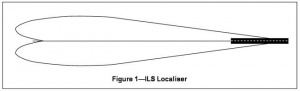
\includegraphics[width=0.4\textwidth, trim={0.2cm 0.5cm 0.2cm 0.1cm}, clip]{img/ILS-LOC}}
	\caption{Rà dio localitzador ILS}
	\label{fig-ils-loc}
\end{figure}

L'altra ràdio és la de pendent de descens o \textit{Glide-Scope} (GS), que permet a
l'aeronau controlar la ràtio de descens durant l'aproximació. (la figura \ref{fig-ils-gs} mostra la
pista d'aterratge i la senyal de ràdio vistes de perfil).

\begin{figure}[!h]
\centering
\fbox{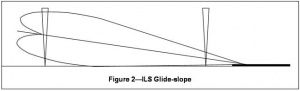
\includegraphics[width=0.4\textwidth, trim={0.2cm 0.5cm 0.2cm 0.1cm}, clip]{img/ILS-GS}}
	\caption{Ràdio Glide-Scope ILS}
	\label{fig-ils-gs}
\end{figure}

El sistema ILS funciona bé i és molt robust, però necessita que les antenes de ràdio
a la pista estiguin instal·lades i funcionin correctament, i avui en dia només els
aeroports i aeròdroms amb més trànsit solen tenir aquest sistema, les pistes més petites i els aeròdroms en llocs remots solen quedar fora de l'equació pel que fa a aterratges
amb ILS.


\section{Planificació}

En aquesta secció descriuré la planificació que vull seguir durant tot el
projecte i el procés que he seguit per arribar-hi a través del mètode
PERT \cite{PERT}.

\subsection{Work Breakdown Structure}
Començaré amb l'Estructura Detallada de Treball o Work Breakdown Structure (WBS)
\cite{WBS}. En la següent llista organitzaré les tasques que considero que són 
necessàries en una estructura jeràrquica de dos nivells:

\begin{enumerate}
    \item Planificar el projecte de forma detallada.
    \item Investigar possibles solucions pel problema plantejat.
    \begin{enumerate}[label*=\arabic*.]
        \item Recopilar una llista de possibles solucions (models de xarxa neuronal).
        \item Investigar pros i contres de cada possible solució
        \item Escollir models a implementar, poden ser més d'un si vull investigar-ne més d'un en profunditat
    \end{enumerate}
    \item Implementar solucions escollides per a una única pista d'aterratge
    \begin{enumerate}[label*=\arabic*.]
        \item Crear datasets o simulació simple per a l'entrenament no supervisat.
        \item Implementar l'algoritme d'entrenament de les solucions escollides.
        \item Provar cada xarxa neuronal i iterar fins aconseguir la precisió desitjada.
    \end{enumerate}
    \item Implementar una simulació complexa per provar el sistema.
    \begin{enumerate}[label*=\arabic*.]
        \item Investigar possibles formes de fer una simulació.
        \item Implementar la simulació de terreny.
        \item Implementar la simulació de l'avió model.
    \end{enumerate}
    \item Provar el sistema sobre la simulació.
    \begin{enumerate}[label*=\arabic*.]
        \item Integrar lògica de control sobre la simulació.
    \end{enumerate}
    \item Investigar integració arduino amb hardware típic d'avions radiocontrol.
    \item Construir un avió model pathfinder.
    \begin{enumerate}[label*=\arabic*.]
        \item Investigar sobre construcció d'avions model.
        \item Construir estructura principal.
        \item Construir electrònica del model.
        \item Proves inicials de vol.
    \end{enumerate}
    \item Construir avió model definitiu, de zero o extenent el model pathfinder.
    \begin{enumerate}[label*=\arabic*.]
        \item Construir estructura principal.
        \item Construir electrònica del model.
        \item Integrar el hardware de control autònom al model.
    \end{enumerate}
    \item Implementar xarxa neuronal i controls en el model.
    \item Provar el model sobre una pista d'aterratge real.
    \begin{enumerate}[label*=\arabic*.]
        \item Sobrevolar la pista controlant l'avió manualment i recopilar les dades necessàries per a poder analitzar les decisions del model després del vol.
        \item Provar l'estabilitat de vol en ràfegues curtes de vol autònom.
        \item Provar aproximacions autònomes i prendre control just abans de l'aterratge.
        \item Provar un aterratge complet.
    \end{enumerate}
    \item Ampliar la xarxa neuronal perquè l'avió pugui aterrar en qualsevol aeroport.
\end{enumerate}

\subsection{Diagrama de Gantt}

Un cop definides totes les tasques les organitzaré en un diagrama de Gantt \cite{Gantt} per poder veure fàcilment la relació que tenen entre elles i el marge de temps que tindré per a realitzar-les.  La figura \ref{fig-gantt} mostra el diagrama de Gantt complet, podem veure que les tasques estan organitzades per setmanes, i hi ha 4 milestones marcades corresponents a les 4 entregues que hauré de fer. També indica el progrés de cada tasca, i per tant aniré actualitzant aquest diagrama a mesura que avanci el projecte.

Aquest diagrama ha estat creat a partir d'aquesta plantilla \cite{GanttLatex} d'Overleaf.

Per comentar una mica l'organització de les tasques, podem veure que hi ha tres fronts principals que es poden fer en paral·lel: la implementació de la xarxa neuronal, la implementació d'una simulació completa on poder fer tests i la creació d'un model físic on poder integrar tot el sistema, i tots tres blocs s'ajunten en les tasques 5 i 9. Tot i que es fan en paral·lel prioritzaré la implementació en software, ja que és el que constitueix el meu Minimum Viable Product, i per tant he reservat més temps del que considero necessari per a la creació de l'avió model, de manera que hi puc dedicar menys temps setmanalment al principi del projecte.


% ######################### DIAGRAMA DE GANTT ############################
\definecolor{barblue}{RGB}{153,204,254}
\definecolor{groupblue}{RGB}{51,102,254}
\definecolor{linkred}{RGB}{165,0,33}
\renewcommand\sfdefault{phv}
\renewcommand\mddefault{mc}
\renewcommand\bfdefault{bc}
\setganttlinklabel{s-s}{}
\setganttlinklabel{f-s}{}
\setganttlinklabel{f-f}{}
\sffamily
\begin{figure*}[!h]
\begin{ganttchart}[
    y unit chart=.75cm,
    canvas/.append style={fill=none, draw=black!5, line width=.75pt},
    hgrid style/.style={draw=black!5, line width=.75pt},
    vgrid={*1{draw=black!5, line width=.75pt}},
    today label font=\small\bfseries,
    title/.style={draw=none, fill=none},
    title label font=\bfseries\footnotesize,
    title label node/.append style={below=7pt},
    include title in canvas=false,
    bar label font=\mdseries\small\color{black!70},
    bar label node/.append style={left=2cm},
    bar/.append style={draw=none, fill=black!63},
    bar incomplete/.append style={fill=barblue},
    bar progress label font=\mdseries\footnotesize\color{black!70},
    group incomplete/.append style={fill=groupblue},
    group left shift=0,
    group right shift=0,
    group height=.5,
    group peaks tip position=0,
    group label node/.append style={left=.6cm},
    group progress label font=\bfseries\small,
    link/.style={-latex, line width=1.5pt, linkred},
    link label font=\scriptsize\bfseries,
    link label node/.append style={below left=-2pt and 0pt}
  ]{1}{19}
  \gantttitle[
    title label node/.append style={below left=7pt and -3pt}
  ]{Setmanes:\quad1}{1}
  \gantttitlelist{2,...,19}{1} \\
  
  % 1 ----------------------------------------------------------
  \ganttgroup[progress=100]{1.Planificar el projecte}{1}{4} \\
  
  % 2 ----------------------------------------------------------
  \ganttgroup[progress=100]{2.Investigar possibles solucions}{1}{4} \\
  \ganttbar[
    progress=100,
    name=WBS2A
  ]{\textbf{2.1} Recopilar possibles solucions}{1}{2} \\
  \ganttbar[
    progress=100,
    name=WBS2B
  ]{\textbf{2.2} Investigar pros i contres}{3}{3} \\
  \ganttbar[
    progress=100,
    name=WBS2C
  ]{\textbf{2.3} Escollir models}{4}{4} \\
  
  % 3 ----------------------------------------------------------
  \ganttgroup[progress=40]{3. Implementar solucions per a una sola pista}{5}{10} \\
  \ganttbar[
    progress=60,
    name=WBS3A
  ]{\textbf{3.1} Crear dataset}{5}{6} \\
  \ganttbar[
    progress=80,
    name=WBS3B
  ]{\textbf{3.2} Implementar algoritme d'entrenament}{7}{9} \\
  \ganttbar[
    progress=10,
    name=WBS3C
  ]{\textbf{3.3} Provar model}{10}{10} \\
  
  % 4 ----------------------------------------------------------
  \ganttgroup[progress=15]{4.Implementar simulació completa}{1}{3} \\
  \ganttbar[
    progress=100,
    name=WBS4A
  ]{\textbf{4.1} Recopilar possibles solucions}{1}{1} \\
  \ganttbar[
    progress=10,
    name=WBS4B
  ]{\textbf{4.2} Implementar simulació de terreny}{2}{3} \\
  \ganttbar[
    progress=0,
    name=WBS4C
  ]{\textbf{4.3} Implementar simulació avió}{2}{3} \\
  
  % 5 ----------------------------------------------------------
  \ganttgroup[
    progress=0,
    name=5
  ]{5.Provar model sobre la simulació i ajustar-lo}{11}{12} \\
  
  % 6 ----------------------------------------------------------
  \ganttgroup[
    progress=90,
    name=6
  ]{6.Investigar integració arduino amb avió rc}{1}{1} \\
  
  % 7 ----------------------------------------------------------
  \ganttgroup[
    progress=20
  ]{7.Crear avió pathfinder}{1}{9} \\
  \ganttbar[
    progress=100,
    name=WBS7A
  ]{\textbf{7.1} Investigar sobre avions radiocontrol}{1}{2} \\
  \ganttbar[
    progress=10,
    name=WBS7B
  ]{\textbf{7.2} Construir estructura principal}{3}{4} \\
  \ganttbar[
    progress=0,
    name=WBS7C
  ]{\textbf{7.3} Construir electrònica del model}{5}{7} \\
  \ganttbar[
    progress=0,
    name=WBS7D
  ]{\textbf{7.4} Proves inicials de vol}{8}{9} \\
  
  % 8 ----------------------------------------------------------
  \ganttgroup[
    progress=0
  ]{8.Construir avió definitiu}{10}{12} \\
  \ganttbar[
    progress=0,
    name=WBS8A
  ]{\textbf{8.1} Construir estructura principal}{10}{10} \\
  \ganttbar[
    progress=10,
    name=WBS8B
  ]{\textbf{8.2} Construir electrònica del model}{11}{11} \\
  \ganttbar[
    progress=0,
    name=WBS8C
  ]{\textbf{8.3} Integrar hardware}{12}{12} \\
  
  % 9 ----------------------------------------------------------
  \ganttgroup[
    progress=0,
    name=9
  ]{9.Implementar Xarxa Neuronal en el model}{13}{13} \\
  
  % 10 ----------------------------------------------------------
  \ganttgroup[
    progress=0
  ]{10.Provar model sobre una pista d'aterratge real}{14}{15} \\
  \ganttbar[
    progress=0,
    name=WBS10A
  ]{\textbf{10.1} Sobrevolar}{14}{14} \\
  \ganttbar[
    progress=0,
    name=WBS10B
  ]{\textbf{10.2} Ràfagues curted de vol autònom}{14}{14} \\
  \ganttbar[
    progress=0,
    name=WBS10C
  ]{\textbf{10.3} Aproximacions completes}{15}{15} \\
  \ganttbar[
    progress=0,
    name=WBS10D
  ]{\textbf{10.4} Aterratge complet}{15}{15} \\
  
  % 11 ----------------------------------------------------------
  \ganttgroup[
    progress=0,
    name=11
  ]{11.Ampliar la xarxa neuronal}{16}{17} \\
  
  \ganttlink[link type=f-s]{WBS2A}{WBS2B}
  \ganttlink[link type=f-s]{WBS2B}{WBS2C}
  
  \ganttlink[link type=f-s]{WBS2C}{WBS3A}
  \ganttlink[link type=f-s]{WBS3A}{WBS3B}
  \ganttlink[link type=f-s]{WBS3B}{WBS3C}
  
  \ganttlink[link type=f-s]{WBS4A}{WBS4B}
  \ganttlink[link type=f-s]{WBS4A}{WBS4C}
  
  \ganttlink[link type=f-s]{WBS3C}{5}
  \ganttlink[link type=f-s]{WBS4C}{5}
  
  \ganttlink[link type=f-s]{WBS7A}{WBS7B}
  \ganttlink[link type=f-s]{WBS7B}{WBS7C}
  \ganttlink[link type=f-s]{WBS7C}{WBS7D}
  
  \ganttlink[link type=f-s]{WBS7D}{WBS8A}
  \ganttlink[link type=f-s]{WBS8A}{WBS8B}
  \ganttlink[link type=f-s]{WBS8B}{WBS8C}
  
  \ganttlink[link type=f-s]{WBS8C}{9}
  
  \ganttlink[link type=f-s]{9}{WBS10A}
  \ganttlink[link type=s-s]{WBS10A}{WBS10B}
  \ganttlink[link type=f-s]{WBS10B}{WBS10C}
  \ganttlink[link type=s-s]{WBS10C}{WBS10D}
  
  \ganttlink[link type=f-s]{WBS10D}{11}
  
  \ganttlink[link type=f-s]{5}{9}
  
  \ganttvrule{Informe 1}{4}
  \ganttvrule{Progrés(I)}{9}
  \ganttvrule{Progrés(II)}{14}
  \ganttvrule{Final}{17}
  
  
\end{ganttchart}
\caption{Diagrama de Gantt del projecte}
\label{fig-gantt}
\end{figure*}

\Needspace{10\baselineskip}
\section{Metodologia}
Per facilitar-me la feina en tot aquest projecte utilitzaré dues eines principals:
\begin{itemize}
    \item{Github per al control de codi font. Tot el meu projecte estarà en aquest repositori de git:
    \href{https://github.com/NarcisNogue/Aterratge-automatic-d-avions-model-basat-en-visio}{Aterratge Automàtic basat en visió}, per a poder tenir un històric de tots els canvis que he fet, poder treballar des de diferents ordinadors i poder compartir el projecte fàcilment. L'únic aspecte del treball que segurament hauré d'excloure del git són els datasets per no superar el límit d'emmagatzematge de 10Gb, però els algoritmes de generació de datasets sí que hi seran.}
    
    \item{Jira per al control de tasques i del temps. He creat un projecte de Jira i hi he afegit les tasques definides a la planificació del projecte, amb una previsió de temps en hores, i a mesura que les vagi fent apuntaré les hores que dedico a cada tasca per veure si el meu ritme de progrés s'adapta a la meva previsió inicial. També utilitzaré el mètode Pomodoro \cite{Pomodoro} de Francesco Cirillo per a les tasques més demandants com aquelles que siguin purament de programació.}
\end{itemize}

Pel que fa a la metodologia de treball, tot el projecte ha quedat repartit en 17 setmanes, i està previst que tot el TFG ocupi al voltant de les 300 hores, per tant cada setmana hauré de dedicar unes 18 hores a treballar. Cada dia de la setmana podré dedicar unes dues hores després de la feina a fer el treball, i per tant els caps de setmana hauria de fer quatre hores cada dia. També he previst una hora de reunió amb el meu tutor cada setmana per comentar el progrés i assegurar que mantinc un bon ritme de treball i comentar la feina de la setmana.


% BIBLIOGRAFIA --------------------------------------------------------
\begin{thebibliography}{9}
\bibitem{ILS}
Instrument Landing System (ILS)
\\\url{https://www.skybrary.aero/index.php/Instrument_Landing_System_(ILS)}
\\Visitat 28-2-2021

\bibitem{Autoland}
Autoland Systems
\\\url{https://www.skybrary.aero/index.php/Autoland}
\\Visitat 1-3-2021

\bibitem{PERT}
La metodologia PERT
\\\url{https://en.wikipedia.org/wiki/Program_evaluation_and_review_technique}
\\Visitat 1-3-2021

\bibitem{WBS}
Work Breakdown Structure
\\\url{https://www.workbreakdownstructure.com/}
\\Visitat 1-3-2021

\bibitem{Gantt}
Diagrama de Gantt en Latex
\\\url{https://www.gantt.com/}
\\Visitat 8-3-2021

\bibitem{GanttLatex}
What is a Gantt Chart?
\\\url{https://es.overleaf.com/project/6045fda53e80236ed63bee8a}
\\Visitat 8-3-2021

\bibitem{Pomodoro}
El mètode Pomodoro
\\\url{http://www.baomee.info/pdf/technique/1.pdf}
\\Visitat 8-3-2021

\end{thebibliography}

\end{document}

© 2021 GitHub, Inc.
Terms
Privacy
Security
Status
Docs
Contact GitHub
Pricing
API
Training
Blog
About
